\documentclass[11pt,a4aper]{article}
\pdfoutput=1

\usepackage[utf8]{inputenc}
%\usepackage{polski}
\usepackage[lf,enc=t1]{berenis}
%\usepackage[main=english,polish]{babel}

\renewcommand{\baselinestretch}{1}
\usepackage[UKenglish]{isodate}
\cleanlookdateon

%%%%% Fonts, symbols, colours, microtypography
\usepackage{amsfonts,amsmath,amssymb,amsthm,mathtools,microtype} % Symbols &microtypography
\usepackage[dvipsnames]{xcolor} % Colours with names -- see https://www.overleaf.com/learn/latex/Using_colours_in_LaTeX for list
\usepackage[noBBpl]{mathpazo} % Palatino, but not for mathbb

%%%%% Figures, tables, lists
\usepackage[labelsep=period,labelfont=bf,justification=centering]{caption}
\usepackage{float,graphicx,subcaption}
\usepackage{enumitem}
\setlist[itemize]{topsep=0ex,itemsep=0ex,parsep=0.4ex}
\setlist[enumerate]{topsep=0ex,itemsep=0ex,parsep=0.4ex}

\usepackage{parskip,fullpage}
\usepackage{thm-restate}
\usepackage[textsize=scriptsize]{todonotes}
\setlength{\marginparwidth}{2cm}%to have larger todonotes
\usepackage{comment}

\usepackage{array}
\usepackage{ifthen}

%%%%% Hyperlinking
\usepackage[hyphens]{url} % Urls together with line breaking them
\usepackage[linktoc=all,hidelinks,colorlinks,unicode=true]{hyperref} % Must be loaded after url
\usepackage[capitalise,compress,nameinlink,noabbrev]{cleveref} % Must be loaded
% after hyperref
\definecolor{color1}{rgb}{.8,.1,.1}
\definecolor{color2}{rgb}{.1,.8,.1}
\definecolor{color3}{rgb}{.1,.1,.8}
\hypersetup{linkcolor={color3},citecolor={color1},urlcolor={purple!70!black}}
\usepackage{hyperref}

\usepackage{listings}
\definecolor{codegreen}{rgb}{0,0.6,0}
\definecolor{codegray}{rgb}{0.5,0.5,0.5}
\definecolor{codepurple}{rgb}{0.58,0,0.82}
\lstdefinestyle{mystyle}{
    backgroundcolor=\color{white},   
    commentstyle=\color{codegreen},
    keywordstyle=\color{magenta},
    numberstyle=\tiny\color{codegray},
    stringstyle=\color{codepurple},
    basicstyle=\ttfamily\footnotesize,
    breakatwhitespace=false,         
    breaklines=true,                 
    captionpos=b,                    
    keepspaces=true,                 
    numbers=left,                    
    numbersep=5pt,                  
    showspaces=false,                
    showstringspaces=false,
    showtabs=false,                  
    tabsize=2
}
\lstset{style=mystyle}


\usepackage{tikz}
\usetikzlibrary{decorations.markings}
\usetikzlibrary{decorations.pathreplacing}
\tikzstyle{classic}=[draw=black,fill = black,inner sep = 1.5pt,circle]

\newtheorem{theorem}{Theorem}
\newtheorem{lemma}[theorem]{Lemma}
\newtheorem{claim}[theorem]{Claim}
\newtheorem*{claim*}{Claim}
\newtheorem{conjecture}[theorem]{Conjecture}
\newtheorem{corollary}[theorem]{Corollary}\newtheorem{proposition}[theorem]{Proposition}
\newtheorem{question}[theorem]{Question}
% \theoremstyle{definition}
\newtheorem{remark}[theorem]{Remark}
\newtheorem{problem}[theorem]{Problem}

\makeatletter
\def\namedlabel#1#2{\begingroup
   \def\@currentlabel{#2}%
   \label{#1}\endgroup
}
\makeatother

\newenvironment{poc}{\begin{proof}[Proof of
    Claim]\renewcommand*{\qedsymbol}{$\blacksquare$}}{\end{proof}}

\newenvironment{csproblem}[1]{\textsc{#1}:\\}{}


\crefname{subsection}{Subsection}{Subsections}

%%%%% Renew commands

\renewcommand{\ge}{\geqslant}
\renewcommand{\le}{\leqslant}
\renewcommand{\geq}{\geqslant}
\renewcommand{\leq}{\leqslant}
% \renewcommand{\eps}{\varepsilon}
\renewcommand{\emptyset}{\varnothing}


\DeclareMathOperator{\og}{og}

%%%%% mathbold and mathcal
\newcommand*{\eps}{\varepsilon}
\renewcommand{\phi}{\varphi}
\newcommand*{\bE}{\mathbb{E}}
\newcommand*{\bN}{\mathbb{N}}
\newcommand*{\bP}{\mathbb{P}}
\newcommand*{\bR}{\mathbb{R}}
\newcommand*{\bZ}{\mathbb{Z}}
\newcommand*{\cF}{\mathcal{F}}
\newcommand*{\cO}{\mathcal{O}}
\newcommand*{\cE}{\mathcal{E}}
\newcommand*{\cI}{\mathcal{I}}
\newcommand*{\cJ}{\mathcal{J}}
\newcommand*{\cR}{\mathcal{R}}
\newcommand*{\cC}{\mathcal{C}}
\newcommand*{\cX}{\mathcal{X}}
\newcommand*{\cG}{\mathcal{G}}
\newcommand*{\cY}{\mathcal{Y}}
\newcommand*{\cB}{\mathcal{B}}
\newcommand*{\cS}{\mathcal{S}}
\newcommand*{\cD}{\mathcal{D}}
\newcommand*{\cM}{\mathcal{M}}
\newcommand*{\cP}{\mathcal{P}}
\newcommand*{\cQ}{\mathcal{Q}}
\newcommand*{\cA}{\mathcal{A}}
\newcommand*{\cU}{\mathcal{U}}
\newcommand*{\orG}{\overrightarrow{G}}
\newcommand*{\orGp}{\overrightarrow{G'}}
\newcommand*{\orH}{\overrightarrow{H}}
\newcommand*{\orHu}{\overrightarrow{H_u}}
\newcommand*{\orHv}{\overrightarrow{H_v}}
\newcommand*{\orGn}{\overrightarrow{G_n}}
\newcommand*{\orGnk}{\overrightarrow{G_{n,k}}}
\newcommand*{\orT}{\overrightarrow{T}}
\newcommand*{\orTn}{\overrightarrow{T_n}}
\newcommand*{\orS}{\overrightarrow{S}}
\newcommand*{\orSn}{\overrightarrow{S_n}}
\newcommand*{\Comb}{\mathrm{Comb}}
\newcommand*{\Col}
{\textsc{3-Col} }
\newcommand*{\MIS}
{\textsc{MIS} }
\DeclareMathOperator{\sq}{\square}

\DeclarePairedDelimiter{\set}{\{}{\}}
\DeclarePairedDelimiter{\abs}{\lvert}{\rvert}
\DeclarePairedDelimiter{\floor}{\lfloor}{\rfloor}
\DeclarePairedDelimiter{\ceil}{\lceil}{\rceil}

% Colors
\newcommand{\colora}{Goldenrod}
\newcommand{\colorb}{SkyBlue}
\newcommand{\colorc}{Sepia}
\newcommand{\colord}{orange}
\newcommand{\colore}{MidnightBlue}
\newcommand{\colorf}{white}
\newcommand{\colorg}{black}

\newcommand{\cola}{\coloredbullet{\colora}}
\newcommand{\colb}{\coloredbullet{\colorb}}
\newcommand{\colc}{\coloredbullet{\colorc}}
\newcommand{\cold}{\coloredbullet{\colord}}
\newcommand{\cole}{\coloredbullet{\colore}}
\newcommand{\colf}{\coloredbullet{\colorf}}
\newcommand{\colg}{\coloredbullet{\colorg}}


  
%%% Comments
\newcommand{\bartosz}[1]{{\color{blue} BW: #1}}
\newcommand{\clement}[1]{{\color{orange} CL: #1}}
\newcommand{\nicolas}[1]{{\color{purple} NT: #1}}
\newcommand{\ugo}[1]{{\color{red} UG: #1}}

\title{Shift graph recognition is NP-complete}

\date{}

\author{
Bartosz Walczak\footnotemark[1] \and 
Cl\'ement Legrand-Duchesne\footnotemark[1]\and
Ugo Giocanti\footnotemark[1] \and
Nicolas Trotignon\footnotemark[2]
}

\begin{document}
\maketitle

\renewcommand{\thefootnote}{\fnsymbol{footnote}} % Make affiliation marks symbols

\footnotetext[1]{Theoretical Computer Science Department, Faculty of Mathematics and Computer Science, Jagiellonian University, Kraków, Poland. U.G. is supported by the National Science Center of Poland
under grant 2022/47/B/ST6/02837 within the OPUS 24 program}
\footnotetext[2]{Univ Lyon, EnsL, UCBL, CNRS, LIP, F-69342, LYON Cedex 07, France}

\renewcommand{\thefootnote}{\arabic{footnote}} % Return to normal footnote symbols



\begin{abstract}
  \todo[inline]{TODO, nicolas test git}
\end{abstract}

\section{Introduction}
\label{sec: intro}
A class of graphs is \emph{hereditary} if it closed under taking induced
subgraphs.  A hereditary class $\mathcal C$ of graph is \emph{$\chi$-bounded} if there
exists a function $f:\mathbb N\to \mathbb N$ such that for each graph $G\in \mathcal C$,
$\chi(G) \le f(\omega(G))$.  A well-known fact is that not all hereditary classes of graphs are
$\chi$-bounded. Even more, there exist triangle-free graphs with arbitrarily large
chromatic number. The first such constructions are due to Zykov \cite{Zyk49} and Blanche Descartes \cite{Descartes}, and among other constructions with such properties, one can also mention Mycielski graphs \cite{Mycielski1955}, shift graphs \cite{EH68}, Burling graphs \cite{Burling},
or some subfamilies of Kneser and Schrijver graphs \cite{lovasz1973Covering, Schrijver}. A common feature of all these graphs is that they all admit explicit constructions, allowing to derive a many interesting structural properties. 
For example, a construction due to Burling turned out
to be a counter-example to several conjectures about algorithms in non-$\chi$
bounded classes~\cite{scott2014Disprove,rzazewski2024Polynomial}. 

% In \cref{tab:complexity}, we review the simplest and most well-known
% constructions of triangle-free graphs of arbitratily large chromatic number.
% Note that most of these constructions (all of them except shift) are usually
% obtained by generating a sequence of triangle-free graphs
% $(G_k)_{k\in \mathbb{N}}$ such that $\chi(G_k) = k$ for all $k$. We turn this
% into a hereditary class by considering the induced subgraphs of the graphs in
% the sequence.  \nicolas{In fact, below, shift graphs are precisely
%   defined as the closure of some sequence, so I would remove ``except
%   shift graphs''. In fact, it is more a matter of presentation, so I
%   rephrase the paragraph below, keep it if you like it.}\ugo{I agree. Also, don't you want to say that we take as a convention from now on that by abuse of notation, when we mean a ``shift'', ``Burling'', etc., then we mean ``induced subgraph of a shift, Burling, etc.\''?}



In \cref{tab:complexity}, we review the simplest and most well-known
constructions of triangle-free graphs of arbitratily large chromatic number.
These constructions are often presented by generating a sequence of triangle-free graphs
$(G_k)_{k\in \mathbb{N}}$ such that $\chi(G_k) = k$ for all $k$. We turn this
into a hereditary class by considering all induced subgraphs of the graphs in
the sequence $(G_k)_{k\in \mathbb N}$. Thus, by abuse of vocabulary, when we say a ``shift/Burling/etc.\ graph'', we mean in particular an induced subgraph of one of the graphs from the sequence $(G_k)_{k\in \mathbb N}$ of shift/Burling/etc.\ graphs (see Section \ref{sec:Prelis} for precise definitions).   


In view of the explicit constructions of each of the aforementioned classes, a natural question is to determine for each of them, whether there exists an efficient (i.e.\ polynomial) algorithm solving the associated membership problem, i.e.\ deciding whether a given graph belongs or not to them. This question has been recently investigated for some of these classes, as well as the complexity of two other natural problems, when restricted to these classes: Maximum Independent
Set (or \MIS for short) and 3-Colouring (see \cref{tab:complexity} for references). The goal of the present paper is to complement these works, and to prove that all three
problems are NP-complete for shift graphs.

% Three problems particularly attracted attention: Recognition, Maximum
% Independent Set and 3-Colouring. The complexity of all of them is known
% for all the classes from \cref{tab:complexity} (where a reference is given),
% except shift graphs. The goal of the present paper is to prove that the three
% problems are NP-complete for shift graphs.
\begin{table}[h!]
  \centering
  \begin{tabular}{|l|c|c|c|}
    \hline
    Graph class & Recognition & Maximum Independent set & 3-Colouring \\
    \hline
    Mycielski & P & NPC \cite{poljak1974Note} & NPC \cite{lovasz1973Covering,maffray1996NPcompleteness} \\
    Zykov & NPC \cite{marin2024Structural} & NPC \cite{marin2024Structural} & NPC \cite{marin2024Structural} \\
    Blanche Descartes & NPC \cite{marin2024Structural} & NPC \cite{marin2024Structural} & NPC \cite{marin2024Structural} \\
    Burling & P \cite{rzazewski2024Polynomial} & P \cite{rzazewski2024Polynomial} & NPC \cite{walczak2025Private}\\
    Twincut & P \cite{bourneuf2025Private} & NPC \cite{bourneuf2025Private} & NPC \cite{bourneuf2025Private} \\
    Shift & NPC [*] & NPC [*] & NPC [*] \\
    \hline
  \end{tabular}  
  \caption{Complexity of Recognition, Minimum independent set and 3-Colouring of
    the main constructions of triangle-free graph of large chromatic number}
  \label{tab:complexity}
\end{table}

Surprisingly, one can observe
from \cref{tab:complexity} that 3-Colouring is NP-complete in all known
constructions of triangle-free graphs of high chromatic number, which motivates
the following conjecture: \nicolas{we could be more general, by saying
``all non-$\chi$-bounded classes (in particular in all triangle-free hereditary graph classes of unbounded
  chromatic number).''}
\begin{conjecture}
  3-Colouring is NP-complete in all triangle-free hereditary graph classes of unbounded
  chromatic number.
\end{conjecture}
\ugo{We should check first whether Kneser/Schrijver constructions do not give a counterexample... Also, do you really want to state it as a Conjecture, and not as a Question?}

For most of the constructions from \cref{tab:complexity} of triangle-free graphs
with high chromatic number, there exist variants producing graphs with
arbitrarily large girth or odd-girth, and unbounded chromatic number. More
precisely, there exist shift graphs, Twincut and Mycielski graphs of arbitrarily
large odd-girth and chromatic number, and Zykov and Blanche Descartes graphs
with arbitrarily large girth and chromatic number. The complexity results of
\cref{tab:complexity} might also hold with this additional condition in these
classes. In the particular case of shift graphs, $k$-iterated shift graphs have
odd-girth at least $2k+3$ but may contain four-cycles. Each of our
NP-completeness results extends to the class of $k$-iterated shift graphs.
Moreover, we prove that shift graphs of girth at least five are 3-colourable,
but that maximum independent set is still NP-complete on shift graphs of
arbitrarily large girth.  
% \paragraph{Abyssal classes}
% In \cite{abrishami2025Burling}, Abrishami et. al. prove that the class of
% Burling graph forms a minimal hereditary class of unbounded chromatic number:
% any proper hereditary subclass of Burling graph has bounded chromatic
% number. The only other known graph class with this property is cliques. At first
% view, the hereditary closures of any construction of triangle-free graphs with
% large chromatic number are natural candidates in the search for other minimal
% hereditary classes of unbounded chromatic number. However, the classes of
% Mycielski, Blanche Descartes, Twincut, Zykov and shift graphs are not minimal.

% Indeed, Mycielski graphs are universal for triangle-free graphs, and
% Blanche Descartes graphs (respectively Twincut graphs or shift graphs) contain
% graphs of arbitrarily large chromatic number and arbitrarily large girth
% (respectively odd girth). Thus none of these classes is
% minimal. Blanche Descartes and Twincut graphs are special cases of Zykov graphs,
% hence Zykov graphs cannot form a minimal hereditary class of unbounded chromatic
% number.

% A class is \emph{abyssal} if it contains no minimal subclass of unbounded
% chromatic number. 

We give in \cref{sec:Prelis} all basic definitions concerning shift graphs, as well as some known characterisations. 
We prove in \cref{sec:MIS} that Maximum independent set (\MIS) is
NP-complete in shift graphs. \cref{sec:3COL} contains a proof that 3-Colouring
(\Col) is NP-complete when restricted to shift graphs and \cref{sec:recognition} shows
that recognising shift graphs is also NP-complete.

\section{Preliminaries}
\label{sec:Prelis}
Unless stated otherwise, all graphs considered in this paper are finite, simple without loops. 
For every integer $n\in \mathbb N$, we use the notation $[n]$ to denote the set $\{1,\ldots,n\}$ of integers.

\subsection{Notations and basic definitions} A digraph $D$ consists of a set $V(D)$ of
vertices and a set $A(D)$ of directed edges denoted $(u,v)$, $uv$ or $u \to v$
and called \emph{arcs}. Given an arc $a=u \to v$, the \emph{head} of $a$ is $v$
and its \emph{tail} is $u$.  An \emph{oriented graph} is a digraph such that for each pair $u,v$ of distinct vertices, $A(D)$ contains at most one of the two arcs $u\to v$ and $v\to u$. The \emph{support} of a digraph $D$ is the undirected graph $G$ obtained
when removing the orientations of the arcs of $D$, that is $V(G) = V(D)$ and
$E(G) = \{\{x,y\} \colon (x,y) \in A(D)\}$. For the sake of notation, we will often use the notation $\orG$ to denote an oriented graph whose support is the unoriented graph $G$. 
We say that a vertex $u$ of a
digraph $D$ is \emph{transitive} if it is neither a source nor a sink. For $k\in \mathbb N$, a
\emph{$k$-walk} (resp.\ \emph{$k$-path}) is a sequence $(v_0,\ldots, v_k)$ of $k+1$ (distinct) vertices such that $v_i\to v_{i+1}$ for each $0\leq i\leq k-1$. Then \emph{length} of a path is defined as its number of edges.
The \emph{$k$-prefix} (resp.\ \emph{$k$-suffix}) of a path $P$
is the subpath obtained when keeping only its $k+1$ first (resp.\ last) vertices.

For each $n\in \mathbb N$, the \emph{transitive tournament of order $n$} is the oriented graph $\orTn$ with vertex set $[n]$, where there is an arc $i\to j$ for each $1\leq i<j\leq n$.

In this paper, the \emph{comb} of length $k$ is the graph $\Comb_k$ obtained from a path on $k$ edges (the \emph{spine} of $\Comb_k$) to which we attach to each vertex an additional pendant edge (such edges are the \emph{teeth} of $\Comb_k$). The comb of length 0 is a single tooth.
 
For a graph $G$, we let $\alpha(G)$ denote the maximum possible size of an independent set of $G$, and
we let $\mathrm g(G)$ and $\og(G)$ denote respectively its \emph{girth} (infimum over the sizes of its cycles) and its \emph{off girth} (infimum over the sizes of its odd cycles). If $D$ is a digraph, we will write $\chi(D)$ to denote the chromatic number of its support graph.

\subsection{Line digraphs}
For a digraph $D$, the \emph{line digraph} $L(D)$ of $D$ is the digraph whose vertices are the arcs
of $D$ and in which there is an arc from $a$ to $b$ if the head of $a$ is the
tail of $b$ in $D$, in other words when $a$ and $b$ are consecutive.
We refer to
$D$ as a \emph{root} digraph of $L(D)$. For $k\in \mathbb N$, the \emph{$k$-iterated line digraph}
$L^k(D)$ of $D$ is then defined recursively by setting $L^k(D) = L(L^{k-1}(D))$ when $k\geq 1$, and
$L^0(D) = D$. Equivalently, when $k\geq 1$, the vertices of $L^k(D)$ are the directed $k$-walks
in $D$ and $L^k(D)$ contains an arc from $a$ to $b$ if the corresponding
directed walks overlap on the $(k-1)$-suffix of $a$ and the $(k-1)$-prefix of
$b$, namely $a = (v_0, \ldots, v_k)$ and $b=(v_1, \ldots, v_{k+1})$ with
$(v_i,v_{i+1}) \in A(D)$ for all $0\leq i\leq k$. Observe that if $D$ is acyclic, then for each $k\geq 2$, the vertex set of $L^k(D)$ also corresponds to the set of $k$-paths of $D$.

The following result of Beineke characterises line digraphs of oriented graphs.
\begin{lemma}[Beineke~\cite{beineke1968Derived}]\label{lem:forbidden_config}
  A digraph $D$ is the line digraph of an oriented graph $\orG$ if and only if the two 
  following conditions are satisfied (see Figure \ref{fig: Beineke}):
  \begin{enumerate}
  \item If $D$ contains three arcs $a$, $b$ and $c$ such that $a$ and $b$ have
    the same tail, and $b$ and $c$ have the same head, then $D$ also contains an
    arc from the tail of $c$ to the head of $a$.
  \item $D$ does not contain four arcs $a$, $b$, $c$ and $d$ such that the tails
    of $a$ and $c$ are identical, the heads of $d$ and $b$ are identical, and
    the head of $a$ (resp. $c$) is the tail of $b$ (resp. $d$).  
  \end{enumerate}
\end{lemma}

\begin{figure}[htb]
  \centering  
  \includegraphics[scale=1]{Line_digraph}
  \caption{The two configurations depicted in Lemma \ref{lem:forbidden_config}.}  
  \label{fig: Beineke}
\end{figure}

% \begin{figure}[ht]
%   \centering
%   \begin{subfigure}{.4\textwidth}
%     \centering
%     \begin{tikzpicture}
%       \node[classic] (1) at (0,0);
%       \node[classic] (2) at (1,.5);
%       \node[classic] (3) at (1,-.5);
%       \node[classic] (4) at (2,0);

%       \draw (1) -> (2);
%       \draw (1) -> (3);
%       \draw (2) -> (4);     
%     \end{tikzpicture}
%     \caption{Consistent neighbourhoods}
%     \label{sfig:config1}
%   \end{subfigure}%
%   \hfill
  
%   \begin{subfigure}{.4\textwidth}
%     \centering
%     \begin{tikzpicture}
%       \node[classic] (1) at (0,0);
%       \node[classic] (2) at (1,.5);
%       \node[classic] (3) at (1,-.5);
%       \node[classic] (4) at (2,0);

%       \draw (1) -> (2);
%       \draw (1) -> (3);
%       \draw (2) -> (4);     
%     \end{tikzpicture}
%     \caption{Forbidden configuration, Condition 2:Consistent neighbourhoods}
%     \label{sfig:config2}
%   \end{subfigure}%
%   \caption{Characterisation of orientations of line digraphs.}
%   \label{fig:config_line_digraph}
% \end{figure}
Note that the second condition forbids parallel arcs in $D'$, while the first
one ensures that all the arcs of $D'$ entering a fixed vertex have identical
out-neighbourhood in $D$. Moreover, note that these two conditions ensure that
the only allowed orientation of a triangle is the cyclic one and the only
allowed orientations of the 4-cycles of $D$ are the cyclic ones and the ones
alternating at each vertex.

Beineke's characterisation gives in particular a easy polynomial time algorithm to recognise line digraphs. On the other hand, Chv\'atal and Ebenegger proved that
deciding if an unoriented graph is the support of a line digraph is NP-complete~\cite{chvatal1990Note}.

\subsection{Shift graphs}
% The class of $k$-shift graphs (or simply shift graphs for $k=2$) is the
% hereditary closure of the graphs $\{G_{n,k} : n \ge 1\}$, that is, all induced
% subgraph of some $G_{n,k}$. Note that this definition is equivalent to saying
% that $k$-shift graphs are the supports of the $(k-1)$-iterated line digraphs of
% all directed acyclic graphs.

The \emph{shift graph sequence} is the sequence of graphs $(G_n)_{n\in \mathbb{N}}$, where $G_n$ is the graph whose vertices are all the ordered pairs $(a_1,a_2)$ of
$[n]$ such that $1 \le a_1 < a_2 \le n$, in which two vertices $a = (a_1, a_2)$
and $b = (b_1, b_2)$ are adjacent if $b_1 = a_2$ (or $a_1 = b_2$). Note that the vertex set of $G_n$ corresponds equivalently to the set of all closed intervals between two distinct integers in $[n]$.
From this
definition, it is straightforward to check that $G_n$ is the support of the line
digraph of the transitive tournament $\orTn$.

The class of \emph{shift graphs} is the hereditary closure of the graphs
$(G_{n})_{n\in \mathbb{N}}$, that is, all induced subgraph of some
$G_{n}$. Note that in the litterature, shift graphs might refer to what we will call later \emph{iterated shift graphs} in this paper.
Observe that every shift graph admits a natural acyclic orientation, obtained when considering the arc $(a,b)\to(b,c)$ for each $1\leq a<b<c\leq n$. We call this orientation the \emph{shift orientation} and denote it with $\orGn$.
% Note that this definition is equivalent to saying that
% shift graphs are the supports of the line digraphs of all acyclic
% digraphs. \ugo{Isn't it what is proved in next lemma?} 
% Equivalently, shift graphs are often defined by the natural acyclic orientation that arises from their interval
% representation: the
% vertices of a shift graph are indexed by intervals $[a,b]$ with
% $1 \le a < b \le n$, and contains an arc from $[a,b]$ to $[c,d]$ if $b =
% c$. 
Since for every oriented graph $\orG$, its line graph $L(\orG)$ is acyclic if and only if $\orG$ is acyclic, Beineke's
characterisation immediately implies the following equivalence:
\begin{lemma}\label{lem:valid}
  A graph is a shift graph if and only if it admits an acyclic
  orientation which is the line digraph of an oriented \ugo{acyclic?} graph.
\end{lemma}

The next lemma is a folklore result. We include its proof as it is simple.

\nicolas{I propose the following lemma, that is more general and
  simplifies stuff later. Note that I use notation og for odd girth, defined with a
  Declaremathoperator. 
  \begin{lemma}\label{lem: line-graph}
For any directed graph $G$, $\chi(L(G)) \geq \log \chi(G)$ and $\og(L(G))
> \og(G)$. 
    \end{lemma}
\begin{proof}
\ugo{The first inequality is proved in 
\cite[Lemma 2.21]{GraphsandHomomorphisms}. I commented the proof}
%   To prove the first inequality, consider a proper colouring $c$ of $L(G)$ using 
%   $k$ colours. Then assign to every vertex $v$ of $G$ the set $S_v$ of
%   all colours with of arcs entering $v$ (with respect to $c$). If
%   $(u,v)$ is an arc of $G$, then as $c$ is a proper colouring,
%   $c(u,v)\notin S_u$, so  $S_u\neq S_v$.  It follows that the mapping
%   $u\mapsto S_u$ defines a proper colouring of $G$ using at most $2^k$ colours, showing $\chi(G) \leq 2^{\chi(L(G))}$ as desired.

  The second inequality is well known and a self contained proof is
  annoying to write. I suggest relying on the equivalence with paths,
  and possibly moving the lemma after the explanations about iterated
  shift graphs. 
\end{proof}
}

As a result all 4-cycles in the natural orientation of a shift graph are
alternating at each vertex and shift graphs are triangle-free. Shift graphs also
have unbounded chromatic number:
\begin{lemma}
  For all $n$, $\chi(G_{2^n+1}) > n$.
\end{lemma}
\ugo{Shall we add a citation?}
\begin{proof}
  Let $K:=\overrightarrow{T_{2^n+1}}$ be the transitive tournament of order $2^n+1$. Note that we then have
  $L(K) = G_{2^n+1}$. Assume for a contradiction that there exists a proper $n$-colouring $\alpha$ of $G_{2^n+1}$. Let
  $\beta: V(K)\to 2^{[n]}$ be the colouring of $K$ such that for each $v\in V(K)$, $\beta(v)$ is the set of colours
  used by $\alpha$ to colour the arcs entering $v$. Then $\beta$ is a
  proper colouring of the support of $K$. To see this, let $u$ and $v$ be two vertices of $K$
  such that $u \to v$ in $K$. As $\alpha$ is a proper colouring of $L(K)$, and as the arcs entering $u$ use the colours in
  $\beta(u)$, the arc $uv$ must be coloured in $\alpha$ by some colour in
  $[n] \setminus \beta(u)$, hence $\beta(v) \neq \beta (u)$. However, the
  support of $K$ is a clique on $2^{n}+1$ vertices, hence it cannot be coloured
  with $2^n$ colours, a contradiction.
\end{proof}

\paragraph{Iterated shift graphs}
For $k\geq 2$, the \emph{$k$-iterated shift graph} $G_{n,k}$ (sometimes referred to as generalised
shift graph, or shift graph) is the graph whose vertices are ordered $(k+1)$-tuples
$(a_0, \ldots, a_k)$ of $[n]$ such that $1 \le a_0 < a_1 < \ldots < a_k \le n$,
in which two vertices $a = (a_0, \ldots, a_k)$ and $b = (b_0, \ldots, b_k)$ are
adjacent if $b_i = a_{i+1}$ for all $i \in [k-1]$ (or $a_i = b_{i+1}$ for all
$i \in [k-1]$). 
From this definition, it is straightforward to check that
$G_{n,k}$ is the support of the $k$-iterated line digraph $L^k(T_n)$ of the transitive
tournament $\orTn$. Note that for each $n\in \mathbb N$, $G_{n,2}$ corresponds exactly to the shift graph $G_n$ defined earlier, and that as before, $G_{n,k}$ admits a natural acyclic orientation, which we call its \emph{shift orientation}, and denote by $\orGnk$. Note also that for each $k\geq 2$, the graph $G_{n,k}$ is a shift graph, we respect to the definition we gave above, i.e.\ it is an induced subgraph of one of the graphs $G_n$. A simple way to see this is to observe that when $k\geq 3$, $G_{n,k}$ is the line digraph of the acyclic oriented graph $L^{k-1}(\orTn)$.
 
The main interest of considering the graphs $G_{n,k}$ is that they give a families of graphs with unbounded chromatic number and arbitrarily large odd girth. More precisely, it is not hard to preve that for every $k\geq 2$ and $n\in \mathbb N$,
$G_{n,k}$ has odd-girth 
at least $2k+3$ (see for example \cite[Lemma 2.22]{GraphsandHomomorphisms}), and that by \cref{lem: line-graph}, $(G_{n,k})_{n \in \mathbb{N}}$ chromatic number at least $\log^{(k)}(n)$, where $\log^{(k)}$ denotes the $k$-iterated logarithm function. The class of the
\emph{$k$-iterated shift graphs} is the hereditary closure of
$(G_{n,k})_{n \in \mathbb{N}}$, or equivalently, the class of all induced subgraphs of
$k$-line digraphs of acyclic digraphs.


Given an acyclic digraph $D$ and an induced subgraph $H$ of $L^k(D)$, we
call \emph{$k$-shift embedding} of $H$ in $D$ any map $\phi$ from the vertices
of $H$ to the $k$-paths of $D$ such that for all $u,v\in V(H)$, $u\to v$ if and
only if the $(k-1)$-prefix of $\phi(v)$ is the $(k-1)$-suffix of $\phi(u)$. %   We
% say that $\phi(u)$ is \emph{private} if for all $v \in V(H) \setminus \{u\}$,
% the $(k-1)$-prefixes of $\phi(u)$ and $\phi(v)$ are different and likewise for
% their $(k-1)$-suffixes.
We say that $\phi$ is \emph{convex} if for every
$u,v,w \in V(H)$ such that $v$ is on a (non-directed) path from $u$ to $w$, then
$V(\phi(u))\cap V(\phi(w)) \subseteq V(\phi(v))$.

\paragraph{Shift trees} We now prove two technical lemmas that we
will use to construct the root graph of some $k$-iterated shift graphs. The first states that for trees, $k$-iterated shift graphs and shift graphs are the same. 

\begin{lemma}\label{lem:shift_tree}
  Let $T$ be a shift graph with shift orientation $\orT$. Then, for all $k\geq 2$, $T$ is also a $k$-iterated shift graph.\\
  More precisely, there exists an acyclic oriented graph $\orG$ and a convex $k$-shift embedding
  $\phi$ of $\orT$ in
  $\orG$. %such that for each leaf $a$ of $T$, $\phi(a)$ is private.
\end{lemma}
\begin{proof}
  We proceed by induction on
  $|V(T)|$. Clearly, if $|V(T)|\leq 1$, then the result is immediate, as if $V(T)$ is empty, then $\orG$ can be chosen as the empty digraph, and if $T$ has a single vertex, then $\orG$ can be chosen as the oriented path of length $k$. We now assume that $|V(T)|\geq 2$.
  
  Let $a$ be a leaf of $T$, and assume without loss of generality that for some $b \in V(T)$ we have
  $a \to b$ in $D$, the case $b\to a$ being symmetric. Let $T':=T-a$, and $\overrightarrow{T'}:=\orT-a$. By induction hypothesis,
  there exists an acyclic oriented graph $\overrightarrow{G'}$ and a convex $k$-shift embedding $\phi'$ of
  $\overrightarrow{T'}$ in $\overrightarrow{G'}$. Let $v$, $w$, $x$, $y$ be the first, second, penultimate and
  last vertex of $\phi(b)$ respectively (with $w=x$ if $k = 2$). Let $Q_b$ be
  the $(k-1)$-prefix of $\phi'(b)$.

  If $b$ is the only vertex of $T'$ with $Q_b$ as the $(k-1)$-prefix of its
  image by $\phi'$, then let $\orG$ be the oriented graph obtained from $\overrightarrow{G'}$ by adding a new
  vertex $u$ with $u \to v$. This creates a $k$-path $P_a$ whose $(k-1)$-suffix
  is the $(k-1)$-prefix of $\phi'(b)$ but of no other $k$-path in
  $\phi'(V(\orT))$. Hence, by defining $\phi(a) := P_a$ and $\phi(c) := \phi'(c)$ for
  all other vertices, $\phi$ is a $k$-shift embedding of $T$ in $G$. The convexity
  of $\phi$ comes from the fact that $\phi'$ was also convex, and that for each $u\in V(T')$, $\phi(u)\cap \phi(a)\subseteq V(Q_b)$. % Moreover, $a$ is the only vertex of $T$ whose image by
  % $\phi$ starts by $a$ and by assumption, $a$ is the only of $T$ whose image by
  % $\phi$ has $(k-1)$-suffix equal to $Q_b$, so $\phi(a)$ is private.
  Thus the
  second part of the lemma holds as well and we can now assume that there exists
  $c \in V(T') \setminus\{b\}$ such that $\phi(c)$ has $Q_b$ as $(k-1)$-prefix
  and ends at $z \in N^+_{G'}(x)$ (see Figure \ref{fig: shiftTree}).
 
 \begin{figure}[htb]
  \centering  
  \includegraphics[scale=1]{shiftTree}
  \caption{Configuration in the proof of Lemma \ref{lem:shift_tree}.}  
  \label{fig: shiftTree}
 \end{figure}

  First, observe that for each $t\in V(G')$ such that $t\to v$ in $\overrightarrow{G'}$,
  we have $tQ_b \notin \phi(V(T'))$, and thus also in particular $b$ is a source in
  $\overrightarrow{G'}$. Indeed, note that otherwise there would exist some node $d \in V(T')$ such that we both have
  $d \to c$ and $d \to b$ in $\overrightarrow{T'}$ (and thus also in $\orT$). In particular, \cref{lem:forbidden_config} would then imply that $a \to b$ in $\orT$, contradicting that $a$ is a leaf of $T$. We now let $\overrightarrow{G''}$ be the oriented graph obtained after duplicating
  the vertex $v$ by creating a vertex $v'$ that is a false twin of $v$ in $\overrightarrow{G'}$, i.e.\ $v'$ has exactly the same out- and in-neighbourhoods as $v$ in $\overrightarrow{G''}$ (note that such operation preserves acyclicity). We define $\psi$ as the map from $V(T')$ to the set of $k$-walks of $G''$ by setting
  $\psi_{|V(T')\setminus \{b\}} := \phi_{|V(T')\setminus \{b\}}$ and define $\psi(b)$ as
  the $k$-path $\phi(b)$ where $v$ was replaced by $v'$. 
  We claim that for any two vertices
  $i,j$ of $V(T')$ we have $i \to j$ in $\overrightarrow{T'}$ if and only if the $(k-1)$-suffix of
  $\psi(i)$ equals to the $(k-1)$-prefix of $\psi(j)$. This is immediate if $i$ and $j$
  are different from $b$, or if $i=b$ because $\psi(i)$ and $\phi(b)$ have the
  same $(k-1)$-suffix. Since $b$ is source in $\overrightarrow{G'}$, the case $b=j$ also
  trivially follows, and as $\phi$ is convex, note that $\psi$ is also convex. We thus just proved that $\psi$ is a convex $k$-shift
  embedding of $\overrightarrow{T'}$ in $\overrightarrow{G''}$ such that $b$ is the only vertex of $\overrightarrow{T'}$ whose
  corresponding $k$-path $\psi(b)$ starts in $v'$. In particular, we are then back in the case of
  the previous paragraph, and can thus conclude the proof.
\end{proof}

\ugo{I hope that I interpretated correctly in the next definition what you meant by ``identifying'' (it was not clear at all for me in a first time).}
In a directed graph $D$, if $u,v$ are two distinct vertices, we let $D/\{u,v\}$ denote the digraph obtained after \emph{identifying} $u$ with $v$, i.e.\  $D/\{u,v\}$ is obtained from $D$ after removing $u,v$ and adding a new vertex $z$, with in-neighbourhood $(N^-_D(u)\cup N^-_D(v))\setminus \{u,v\}$ and
out-neighbourhood $(N^+_D(u)\cup N^+_D(v))\setminus \{u,v\}$. Note that if $D=\orH$ is an oriented graph, in which $N_H(u)$ and $N_H(v)$ are disjoint, then $D/\{u,v\}$ is also an oriented graph. The next lemma shows that in this case, $k$-shift embeddings are also preserved.

\ugo{I do not  understand at all the next lemma... Could you define what it does mean to identify $\phi(u)$ with $\phi(v)$? Is $G$ oriented?}

\begin{lemma}\label{lem:gluing}
  Let $\phi$ be a $k$-shift embedding of $H$ in $G$ and let $u,v$ be two
  vertices of $H$ with $\phi(N(u))$ and $\phi(N(v))$ vertex disjoint, such that
  there is no directed path from $u$ to $v$ or vice-versa. Then $\phi$ is a
  $k$-shift embedding of the graph obtained from $H$ by identifying $u$ with $v$
  into the graph obtained from $G$ by identifying $\phi(u)$ with $\phi(v)$.
\end{lemma}

\begin{proof}
  First, note that this identification is well-defined because $\phi(N(u))$ and
  $\phi(N(v))$ are vertex-disjoint, in particular, the neighbours of $u$ and $v$
  are preserved. This identification creates no directed cycle because there are
  no directed paths between $u$ and $v$ in $H$.
\end{proof}

\section{Maximum independent set problem}\label{sec:MIS}

Given a graph $G$ and an integer $\ell\in \mathbb N$, denote $G^{\ast\ell}$ the graph obtained by subdividing $\ell$
times each edge of $G$. In particular, we have $G^{\ast 0}=G$. 

\begin{lemma}[\cite{poljak1974Note}]\label{lem:subdivision_MIS}
  For every graph $G$ and every even integer $\ell\geq 0$, we have
  $\alpha(G^{\ast\ell}) = \alpha(G) + \frac{\ell}2|E(G)|$.
\end{lemma} 

\begin{proposition}
  For any $k$ and $\ell$, \MIS is NP-complete when restricted to the class of $k$-iterated shift
  graphs of girth at least $\ell$.
\end{proposition}
\begin{proof}
  We fix $k,\ell\in \mathbb N$ and show that \MIS on general graphs admits a polynomial time reduction to \MIS when restricted to the class of $k$-iterated shift graphs. Let $G$ be a connected graph and assume that $[n]=V(G)$. We claim that $G^{*\ell}$ is a $k$-iterated shift graph of girth
  at least $\ell$. By \cref{lem:subdivision_MIS}, this will imply directly the result. \ugo{Don't you need some condition on $k$? If $\ell=0$, the result does clearly not hold, did I miss something? And shouldn't $\ell$ be even?}
  To prove our claim, consider the following
  acyclic digraphs. Given $i \in \{0, \dots k\}$, let $H_{i,\ell}$ be the
  digraph constructed as follows. For each edge $e=uv$ of $G$ with $u<v$,
  let $P_e$ be a directed $(i+\ell+1)$-path. For each $v$, identify the
  $i$-prefixes of all the paths $P_{vw}$ with $v<w$ and the $i$-suffixes of all
  the paths $P_{uv}$ with $u<v$. In particular, we have
  $H_{0,\ell} = G^{*\ell}$.  We also have $L(H_{i, \ell}) =
  H_{i-1,\ell}$. \ugo{Maybe that I did not understand smg, but I disagree with this equality.} Indeed, the line digraph operation maps each $(i+\ell+1)$-path
  $P_{uv}$ of $H_{i,\ell}$ to an $(i+\ell)$-path and the identified sections of
  length $i$ in $H_{i,\ell}$ to the identified sections of length $i-1$ of
  $L(H_{i, \ell})$. So $L^k(H_{k, \ell}) = H_{0,\ell}= G^{*\ell}$, which proves
  that $G^{*\ell}$ is a $k$-iterated shift graph and concludes this proof.
\end{proof}

\section{3-Colouring shift graphs}\label{sec:3COL}
\begin{theorem}\label{thm:3col}
  For any $k\geq 2$, \Col is NP-complete when restricted on the class of $k$-iterated shift graphs (and
  \emph{a fortiori} in shift graphs of odd-girth at least $k$).
\end{theorem}
\begin{proof}
  We design a polynomial time reduction from \Col on general graphs to \Col on $k$-iterated
  shift graphs. For simplicity, we first describe our reduction for shift graphs
  before adapting it to $k$-iterated shift graphs, as the latter case is more technical, but the ideas are essentially identical. We will equivalently view proper colourings
  of $L(\orG)$ as arc-colourings of $\orG$, that is an assignement of colors to $A(G)$
  such that $u\to v$ and $v\to w$ have distinct colors for all $u,v,w \in V(G)$.

\paragraph{The gadget H}
  We construct an acyclic oriented graph $\orH$ such that $\chi(L(\orH))=3$, having a
  marked vertex $x$ with the following property: in any 3-arc-colouring of $\orH$
  the set of arcs entering $x$ uses exactly two colours. 


\nicolas{I think everything works fine by taking a graph $T$ with
  odd girth $k$ and a minimum number of vertex $n$ and such that
  $\chi(L(T)) = 4$. Then, we don't have to consider higher odd girths
  separatly. The fact that $T$ comes from a tournament is not
  essential. Very little has to be changed in the proof.}

  
  Consider the minimum value of $n\in \mathbb N$ such that the transitive $n$-vertex tournament $\orTn$ satisfies
  $\chi(L(\orTn))=4$. Let $v_{n-1}$ and $v_n$ respectively denote the vertices of $\orTn$ with respective in-degrees
  $n-2$ and $n-1$. % Let $S_n$ be the subgraph of $T_n$
  % obtained by removing all the arcs $uv_n$ with $u \in V(G) \setminus
  % \{v_{n-1},v_n\}$. Given an arc-colouring $\alpha$ of $S_n$,
  % let $\beta$ be the arc-colouring of $T_n$ such that $\beta(xy) = \alpha(xy)$
  % if $xy\in A(S_n)$ and $\beta(uv_n) = \alpha(uv_{n-1})$ for all
  % $u \in V(T_n) \setminus \{v_{n-1},v_n\}$. The arc-colouring $\beta$ is
  % proper because $uv_n$ and $uv_{n-1}$ are twins in $L(T_n)$. Since $\alpha$ and
  % $\beta$ use the same amount of colours and $S_n$ is a subgraph of $T_n$, we
  % have $\chi(L(S_n)) = \chi(L(T_n)) = 4$.
  Let $\orH$ be the graph obtained from $\orTn$ by iteratively removing all the arcs entering $v_{n-1}$
  until the chromatic number of its line digraph drops to three. Note that
  $\overrightarrow{S_n} := \orTn-\{uv_{n-1} : u \in V(T_{n})\setminus\{v_{n-1},v_{n}\}\}$ is the
  transitive tournament on the vertices $V(T_n)\setminus \{v_{n-1}\}$, with an
  additional vertex $v_{n-1}$ whose only incident arc ends in the sink $v_n$. Thus
  $\orSn$ is 3-arc-colourable, and $\orH$ is well defined.


  % \nicolas{Typos in the paragraph below: line 5, it should be $\{1,
  %   3\}\setminus c$ and line 7 it should be colour different from 2
  %   and $c$.}

  
  Let $uv_{n-1}$ be the last arc removed in the construction of $\orH$. We thus have
  $\chi(L(\orH + uv_{n-1})) = 4$ and $\chi(L(\orH)) = 3$. Let $\phi$ be a proper
  3-colouring of $L(\orH)$, where $v_{n-1}v_n$ is without loss of generality
  coloured 1. The arcs entering $v_{n-1}$ cannot use the colour 1, so they use
  at most two colours. Suppose that they are all using the same colour, say
  2 (see Figure \ref{fig: GadgetH}). Let $c := \phi(uv_n)$ (note that $c$ is well defined as $u\to v_n$ is an arc of $\orH$) and $\beta$ be the 3-colouring of $L(\orH+uv_{n-1})$
  such that $\beta(uv_{n-1}):= c$,
  $\beta(v_{n-1}v_n) \in \{1,3\} \setminus \{c\}$ and $\beta(xy) = \phi(xy)$
  for all other arcs. The arc-colouring $\beta$ uses three colours like $\phi$ and we claim that it
  is a proper colouring of $L(\orH+uv_n)$. 
  As $\phi$ is proper, it suffices to check 
  that the colourings of the arcs $uv_{n-1}$ and $v_{n-1}v_n$ do not create a monochromatic edge. As $v_n$ is a sink, and as $uv_n$ was colored with $c$ by $\phi$, note that the arc $uv_{n-1}$ cannot have a neighbour of colour $c$ in $L(\orH+uv_n)$.
  Moreover, $v_{n-1}v_n$ is the only arc of $L(\orH+uv_n)$ starting in $v_{n-1}$, and uses a colour different from 2 and $c$, showing that $\beta$ is a proper $3$-colouring. This contradicts 
  $\chi(L(\orH+uv_n))=4$. We thus deduce that the set of arcs entering $v_{n-1}$ in $H$ use both the colours 2 and 3.
  To sum up, $\orH$ is 3-colourable and in each 3-arc-colouring of $\orH$, the arcs
  entering the marked vertex $x:=v_{n-1}$ use two different colours.
  
\begin{figure}[htb]
  \centering  
  \includegraphics[scale=1]{GadgetH}
  \caption{In red, the coloration $\phi$ depicted in  the first part of the proof of \cref{thm:3col}.}  
  \label{fig: GadgetH}
\end{figure}

  
  
  % We construct an acyclic oriented graph $H$ with two marked arcs $e$ and $f$ with a
  % common marked head $x$ such that any 3-arc-colouring of $H$ colours $e$ and
  % $f$ differently. Let $H$ be the oriented graph on ten vertices $u_0, \ldots, u_8$ and
  % $x$ constructed as follows (see \cref{fig:gadget_3col}). For each
  % $i, j \in \{0, \ldots, 6\} \cup \{8\}$, add the arc $u_i \to u_j$ if
  % $i < j < i+5$ (in black in \cref{fig:gadget_3col}). Add also the arcs
  % $u_3 \to u_7$, $u_4 \to u_7$ and $u_5 \to x$, $u_6 \to x$ (respectively in red
  % and blue in \cref{fig:gadget_3col}). In $H$, $x$ is a
  % sink and a computer check shows that $H$ is 3-arc-colourable, and that all
  % 3-arc-colourings of $H$ use distinct colours on $u_5 \to x$ and $u_6 \to
  % x$ (see \cref{sec:computer_check}).

  % \begin{figure}[h!]
  %   \centering
  %   \begin{tikzpicture}[decoration={
  %       markings,
  %       mark=at position 0.5 with {\arrow[scale=1.5]{>}}}
  %     ]
  %     \foreach \i in {0,...,8}{
  %       \node[classic] (\i) at (\i,0) {};
  %       \node[below left] at (\i) {$u_{\i}$};
  %     }

  %     \node[classic] (x) at (5.5,-1.5) {};
  %     \node[below left] at (x) {$x$};

  %     \foreach \i in {0,...,6}{
  %       \pgfmathsetmacro{\a}{int(\i+1)}
  %       \pgfmathsetmacro{\b}{min(int(\i+4),8)}
  %       \foreach \j in {\a,...,\b}{
  %         \ifthenelse{\j = 7}{}
  %         {\draw (\i) edge[bend left=(\j-1-\i)*20, postaction=decorate] (\j);}
  %       }
  %     }
  %     \foreach \i in {3,4}{
  %       \draw[color1] (\i) edge[bend left=(6-\i)*20, postaction=decorate] (7);
  %     }
  %     \draw[color3,postaction=decorate] (5) -- (x);
  %     \draw[color3,postaction=decorate] (6) -- (x);
  %   \end{tikzpicture}
  %   \caption{The gadget $H$}
  %   \label{fig:gadget_3col}
  % \end{figure}

  \paragraph{Constructing the shift graph}
  Let $G$ be a graph. We contruct an acyclic oriented graph $\orGp$ such that
  $\chi(G) \le 3$ if and only if $\chi(L(\orGp)) \le 3$ as follows. Fix an arbitrary total order $<$ on the
  vertex set of $G$ and for each vertex $u$ of $G$, take a copy $\orHu$
  of $\orH$, with an arc $e_u:=x_u \to y_u$ starting in the marked vertex $x_u$ of
  $H_u$ and ending in a new pendant vertex $y_u$. For each edge $uv \in E(G)$, with
  $u < v$, add the arc $x_u \to x_v$ (see \cref{fig:NP-col}). The oriented graph
  $\orGp$ constructed is acyclic because each copy $\orHu$ of $\orH$ is acyclic and
  separated from the rest of $G'$ by the cut vertex $x_u$, and the additional
  edges can be ordered acyclically following the order on the vertices of
  $G$. Therefore $L(\orGp)$ is a shift graph. 
  
  We will now show that $G$ is 3-colourable if and only if $L(\orGp)$ is 3-colourable.

  \begin{figure}[h!]
    \begin{subfigure}[t]{.3\textwidth}
      \centering
      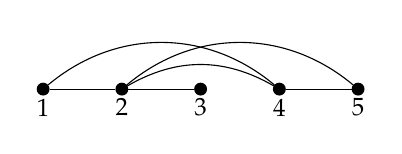
\begin{tikzpicture}
        \foreach \i in {1,2,3,4,5}{
          \node[classic] (a\i) at (\i,0) {};
          \node[below] at (a\i) {\small $\i$};
        }
        \draw (a1) -- (a2) -- (a3) (a4) -- (a5);
        \draw (a2) edge[bend left] (a4);
        \draw (a2) edge[bend left=40] (a5);
        \draw (a1) edge[bend left=40] (a4);
      \end{tikzpicture}
      \caption{A graph $G$}
    \end{subfigure}
    \hfill
    \begin{subfigure}[t]{.65\textwidth}
      \centering
      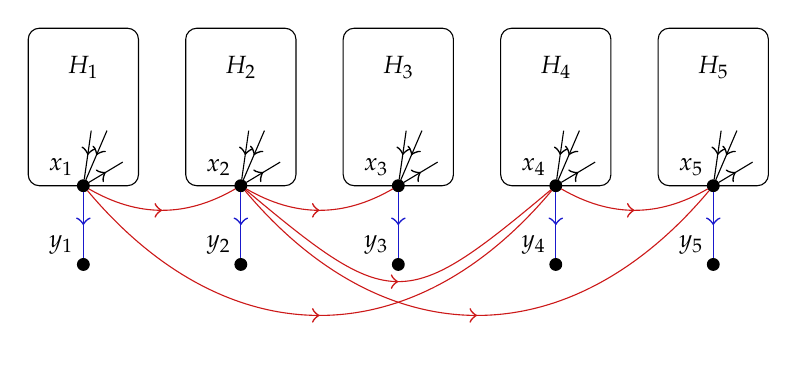
\begin{tikzpicture}[decoration={
        markings,
        mark=at position 0.5 with {\arrow[scale=1.5]{>}}}
      ]
        \foreach \i in {1,2,3,4,5}{
          \begin{scope}[shift={(2*\i,0)}]
            \draw[rounded corners] (-.2,0) rectangle (1.2,2);
            \node[classic] (x\i) at (.5,0) {};
            \node[above left] at (x\i) {\small $x_{\i}$};
            \node[classic] (y\i) at (.5,-1) {};
            \node[above left] at (y\i) {\small $y_{\i}$};
            \node (H\i) at (.5,1.5) {\small $H_{\i}$};
            \draw[postaction=decorate] (.6,.7) -- (x\i);
            \draw[postaction=decorate] (.8,.7) -- (x\i);
            \draw[postaction=decorate] (x\i) -- (1,.3);

            \draw[color3,postaction=decorate] (x\i) -- (y\i);
          \end{scope}
        }

        \draw[color1] (x1) edge[bend right,postaction=decorate] (x2);
        \draw[color1] (x2) edge[bend right,postaction=decorate] (x3);
        \draw[color1] (x4) edge[bend right,postaction=decorate] (x5);
        \draw[color1] (x2) edge[bend right=40,postaction=decorate,looseness=1.6] (x4);
        \draw[color1] (x2) edge[bend right=50,postaction=decorate,looseness=1.2] (x5);
        \draw[color1] (x1) edge[bend right=50,postaction=decorate,looseness=1.2] (x4);

      \end{tikzpicture}
      \caption{The oriented graph $\orGp$ constructed. The blue arcs $x_i \to y_i$
        correspond to the vertices of $G$ and the red arcs to its edges.}
    \end{subfigure}
    \caption{Constructing an equivalent shift graph.}
    \label{fig:NP-col}
  \end{figure}

  \paragraph{Equivalence of the instances}
  Assume that there exists a 3-colouring $\alpha$ of $G$. Colour each arc
  starting in $x_u$ with the colour of $u$ in $\alpha$. At this stage it remains
  only to colour the copies of $H$. Let $\beta$ be a 3-arc-colouring of $H$. For
  each copy $H_u$, permute the colours of $\beta$ such that the arcs entering
  $x_u$ use the two colours different from $\alpha(u)$. The resulting colouring
  is a 3-arc-colouring of $G'$. Indeed, at each $x_v$, all the arcs starting in
  $x_v$ have an identical colour $\alpha(v)$, and the arcs entering $x_v$ are
  either coming from the copy $H_v$ or of the form $x_u \to x_v$ for some
  $u < v$, in both case they use colours different from $\alpha(v)$. Thus
  $L(G')$ is 3-colourable.

  Conversely, in a proper 3-arc-colouring of $G'$, by design of $H$, all the
  arcs starting in $x_u$ are coloured identically. Colour $u$ with this
  colour. Given any edge $uv$ in $E(G)$ with $u<v$, the colour of $u \in V(G)$
  is the colour of $x_u\to x_v$ which differs from the colour of $x_v \to y_v$,
  that is the colour of $v \in V(G)$. Thus $G$ is 3-colourable.

  \paragraph{$k$-iterated shift graphs}
  To adpat our reduction to $k$-iterated shift graph, we will first need to
  change our gadget. Given a $k$-iterated line digraph $G_2$ of an oriented
  graph $G_1$, we will for convenience see the $k$-colourings of $G_2$ as
  $k$-colourings of the $k$-paths of $G_1$ such that the $k$-paths
  $u_0\dots u_k$ and $u_1\dots u_{k+1}$ are coloured differently.

  For our gadget, we construct an acyclic oriented graph $H$ such that
  $\chi(L^k(H))=3$, with a marked $(k-1)$-path $X$ with the following property:
  in any 3-colouring of $L^k(H)$, the set of $k$-paths with suffix $X$ use
  exactly two colours.

  Consider the minimum $n$-vertex transitive tournament $T_n$ such that
  $\chi(L^k(T_n))=4$. For each $i \in [n]$, let $v_i$ be the vertex of indegree
  $i-1$ in $T_n$. % Let $S_n$ be the subgraph of $T_n$ obtained by removing all
  % the arcs $v_jv_{n-i}$  for all $i \in \{0, \dots, k-1\}$ and 
  % $j<n-i-1$. The oriented graph $S_n$ consists of a transitive tournament on the
  % vertices $\{v_i : i \in [n-k]\}$, with a $k$-path on the vertices
  % $v_{n-k}, \dots v_n$. Let $\phi$ be the following map from the $k$-paths of if
  % $xy\in A(S_n)$ and $\beta(uv_n) = \alpha(uv_{n-1})$ for all
  % $u \in V(T_n) \setminus \{v_{n-1},v_n\}$. The arc-colouring $\beta$ is proper
  % because $uv_n$ and $uv_{n-1}$ are twins in $L(T_n)$.  $T_n$ to the $k$-paths
  % of $S_n$. For all $k$-paths $P$ of $S_n$, $\phi(P) = P$. Any other $k$-path
  % $P$ of $T_n$ is the concatenation of a $i$-path $Q$ on the vertices of
  % $\{v_j : j < n-k\}$ and a $k-i-1$-path on vertices of
  % $\{v_j: \in \{n-k, \dots n\}$. For such paths, $\phi(P)$ is the concatenation
  % of $Q$ with $v_{n-k}, \dots v_{n-k+i-1}$. In particular, note that $P$ and
  % $P'$ are consecutive in $T_n$, \emph{i.e.} the suffix of length $k-1$ of $P$
  % is the prefix of length $k-1$ of $P'$, then $\phi(P)$ and $\phi(P')$ are
  % consecutive in $S_n$. Thus, given a colouring $\alpha$ of $L^k(S_n)$, the
  % colouring $\beta$ of $L^k(T_n)$ such that $\beta(P) = \alpha(\phi(P))$ for all
  % $P$ is a proper colouring. Since $\alpha$ and $\beta$ use the same amount of
  % colours and $S_n$ is a subgraph of $T_n$, we have
  % $\chi(L(S_n)) = \chi(L(T_n)) = 4$.
  Let $H$ be the subgraph of $T_n$ obtained by removing vertices of the form
  $v_iv_{n-k}$ with $i<n-k$ until the chromatic number of its $k$-iterated line
  digraph drops to three. Note that $S_n = T_n-\{v_iv_{n-k} : i <n-k\}$ is the
  transitive tournament on the vertices
  $v_1, \dots v_{n-k-1}, v_{n-k+1} \dots v_n$ with the additional vertex
  $v_{n-k}$ and all arcs of the form $v_{n-k}v_j$ with $j>n-k$. As such,
  $L^k(S_n)$ is isomorphic to the $k$-iterated line digraph of the transitive
  tournament on $n-1$ vertices, with one additional isolated vertex,
  corresponding to the $k$-path $v_{n-k}, \dots v_n$. So $L^k(S_n) = 3$ and $H$
  is well defined. Let $uv_{n-k}$ be the last arc removed in the construction
  of $H$, we have $\chi(L^k(H))= 3$ and $\chi(L^k(H+uv_{n-k}))=4$.

  Let $\alpha$ be a 3-colouring of $L^k(H)$, and without loss of generality
  assume that the $k$-path $v_{n-k}, \dots v_n$ is coloured 1 by $\alpha$. We
  will now argue that the set of $k$-paths with suffix $X:=v_{n-k}\dots v_{n-1}$
  is coloured with the colours 2 and 3, and thus that all the $k$-paths with
  prefix $X$ in the second part of the reduction are coloured 1. First, since
  $P=v_{n-k}\dots v_n$ is coloured 1 and is the only $k$-path starting in
  $v_{n-k}$, the $k$-paths of $H$ with suffix $X$ are coloured using a subset of
  $\{2,3\}$.

  Suppose that they all use the same colour, say 2.  Let $c$ be the colour of
  the $k$-path $uv_{n-k+1} \dots v_n$. Let $f$ be the map from the
  $k$-paths of $H+uv_{n-k}$ to $H$ defined as follows. For each $k$-path $P$
  avoiding the arc $uv_{n-k}$, we let $f(P) =P$. Given a $k$-path $P$ passing by
  $uv_{n-k}$, let $Q$ its prefix ending at $u$ and $R$ its suffix starting
  at $v_{n-k}$ and let $f(P)$ be the concatenation of $Q$ and
  $v_{n-k+1}, \dots v_{n-k+1+q}$ where $q$ is the length of $Q$. In particular,
  if $P$ and $P'$ are consecutive in $T_n$, then so are $f(P)$ and
  $f(P')$. Let $\beta$ be the 3-colouring of $L(H+uv_{n-k})$ defined as
  follows. For any $k$-path $P$ without $X$ as suffix or prefix, let
  $\beta(P) = \beta(f(P))$. Any $k$-path $P$ with suffix $X$ in
  $H+uv_{n-k}$ is either a $k$-path of $H$, in which case $\alpha(P)=2$ and we
  define $\beta(P) = 2$, or the $k$-path $uv_{n-k}\dots v_{n-1}$, in which
  case we let $\beta(P) = \alpha(uv_{n-k+1}\dots v_n) = c$. The only remaining
  $k$-path where $\beta$ is undefined is the path $P = v_{n-k} \dots v_n$ with
  $X$ as prefix. By construction the indicent paths in $L^k(H+uv_{n-k})$ are
  colored 2 and $c$, so we can colour this path with a colour from
  $\{1,3\}\setminus\{c\}$. The colouring $\beta$ is a proper 3-colouring of
  $L^k(H+uv_n)$, which contradicts $\chi(L^k(H+uv_{n-k})$. So the $k$-paths
  with suffix $X=v_{n-k}\dots v_{n-1}$ use the colours 2 and 3 in $\alpha$. To
  sum up, $L^k(H)$ is 3-colourable and in each 3-colouring of $L^k(H)$, the
  $k$-paths with prefix $X$ use two different colours.

  We finish the reduction in a similar way as for shift graphs. Let $G$ be a
  graph, with an arbitrary order on its vertices. For each vertex $u$ of $v$,
  take a copy $H_u$ of $H$ and a new vertex $y_u$, and attach an arc $x_uy_u$ to
  the last vertex $x_u$ of the marked $(k-1)$-path $X_u$ of $H_u$. For each edge
  $uv$ of $G$ with $u<v$, add a pending arc $x_uz_{uv}$ to $x_u$ and identify
  the marked $(k-1)$-path $X_v$ with the $(k-1)$-path formed by concatenating
  the $(k-2)$-suffix of $X_u$ with $z_{uv}$. As a result, the $k$-paths
  $X_ux_v$ and $X_vy_v$ are consecutive.  The oriented graph $G'$ constructed is
  acyclic because each the copies $H_u$ are acyclic and ordered following the
  order of the vertices of $G$. We consider the subgraph $L$ of $L^k(G')$
  induced by the $k$-paths that contain at most one arc between different
  vertices labelled $x_u$ for some $u$.

  We claim that $L$ is 3-colourable if and only if $G$ is 3-colourable. Let
  $\alpha$ be a 3-colouring of $G$. Let $\beta$ be the 3-colouring of $L$
  defined as follows. First, for each $u \in V(G)$, colour each $k$-path of $G'$
  with penultimate vertex equal to $x_u$ with the colour $\alpha(u)$. Each
  remaining $k$-path of $L$ is fully contained in some $H_u$ for some $u$
  because we removed from $L$ the $k$-paths containing more than one arc between
  different vertices labelled $x_u$ for some $u$. For each $u$, all the
  $k$-paths with suffix $X_u$ of $H_u$ are identically coloured, so one can
  permute the colours in a fixed 3-colouring of $L^k(H)$ to colour
  $L^k(H_u)$. Two consecutive $k$-paths of $L$ are either both contained in some
  $H_u$, or with suffix and prefix equal to some $X_u$, or with prefix equal to
  some $X_u$ and formed by the $(k-2)$-suffix of $X_u$ concatenated with
  $x_vy_v$ for some $v>u$ with $uv \in E(G)$. In either case, their colours are
  different by construction. Conversely, given a proper 3-colouring $\beta$ of
  $L$, let $\alpha$ be the colouring of $G$ such that for each $u$, $\alpha(u)$
  is the colour in $\beta$ of the $k$-path with prefix $X_u$ finishing in
  $y_u$. By design of $H$, all $k$-path with prefix $X_u$ are identically
  coloured and so $\alpha(u)$ and $\alpha(v)$ are different for each
  $uv \in E(G)$ with $u<v$, because the paths $X_ux_v$ and $X_vy_v$ are
  consecutive by construction and
  $\alpha(u) = \beta(X_ux_v) \neq \beta(X_vy_v) = \beta(v)$.
\end{proof}

We now prove that if one restricts to shift graphs of large girth (and not large
odd-girth as in \cref{thm:3col}), 3-colouring becomes a trivial problem.
\begin{proposition}
  All shift graphs of girth at least five are 3-colourable.
\end{proposition}
\begin{proof}
  Let $G$ be a shift graph of girth at least five and let $H$ be a root oriented graph
  of $G$. The vertices of $H$ have either in or out-degree at most one, because
  a vertex with in and out degree at least two produces a four-cycle in the line
  digraph. We partition the vertices of $H$ in two subsets: $X$ contains the
  vertices of indegree at most one, and $Y$ the remaining vertices, which have
  outdegree at moste one. We partition the arcs of $H$ in two subsets: $A$
  contains the arcs entering $X$ or starting in $Y$, and $B$ contains the other
  arcs, which start in $X$ and end in $Y$. The arcs of $B$ are independent so
  they can be coloured with one colour, say 1. We claim that the arcs of $A$
  form a forest, so they can be coloured with two additional colours, which
  results in a 3-arc-colouring of $H$. Let $A_1$, $A_2$ and $A_3$ the subgraphs
  formed by the arcs of $A$ that respectively connect two vertices of $X$,
  connect to vertices of $Y$, start in a vertex of $Y$ and end in a vertex of
  $X$. Because $H[X]$ has indegree at most one, the subgraph $A_1$ forms a
  forest of trees directed towards their root. Likewise, $A_2$ forms a forest of
  trees directed away their root. Because $X$ and $Y$ have respectively in and
  outdegree at most one, $A_3$ forms a matching between the roots of these two
  forests. Hence $A$ form a forest, which concludes the proof.
\end{proof}
\section{Recognising shift graphs}\label{sec:recognition}

By Schaefer's dichotomy theorem~\cite{schaefer1978Complexity}, the following
problem is NP-complete.

\begin{csproblem}{Monotone Not all equal (MNAE3SAT)}
  Given a monotone 3-CNF formula $\phi$ (in conjonctive normal form with three
  non-negated variables per clause), recognise if there exists a valuation to
  the variables such that each clause of $\phi$ contains true and false variables.
\end{csproblem}



\begin{theorem}
  Let $k \ge 1$. Recognising a $k$-iterated shift graph (or equivalently, the
  support of the $k$-iterated line digraph of
  an acyclic oriented graph) is an NP-complete problem.
\end{theorem}
\begin{proof}
  % Here again, we first explain the reduction to shift graphs before adapting it
  % to iterated shift graphs.
  Let $k \in \mathbb{N}$. We reduce \textsc{MNAE3SAT} to the $k$-iterated shift
  graph recognition problem.  Let $\phi$ be a monotone 3-CNF formula with $m$
  clauses. We build a graph $G_\phi$ that is a $k$-iterated shift graph if
  $\phi$ is a valid instance of \textsc{MNAE3SAT}, but is not a shift graph (and
  \emph{a fortiori} not a $k$-iterated shift graph) if $\phi$ is not a valid
  instance of \textsc{MNAE3SAT}.

  \paragraph{Gadgets}
  We first describe the gadget used for the variables. Let $H$ be the 4-sun,
  that is the graph on eight vertices composed of a 4-cycle with one pending
  edge attached to each of the vertices of the cycle. For each variable $x$,
  consider the gadget composed of a path on $8m+1$ vertices
  $u_x^{-1}, \dots, u_x^{8m-1}$ in which for each $i \in \{0, \ldots, 4m-1\}$ we
  connect $u_x^{2i}$ to the extremity first vertex of the spine of a comb
  of length $k+1$. Denote $v_x^{2i}$ the last vertex of the spine of this
  comb and $w_x^{2i}$ the vertex adjacent to $v_x^{2i}$ via the last tooth.
  Connect each $u_x^{2i}$ to a distinct copy of $H$ via one of its vertices of
  degree three that we will call $t_x^{2i}$ (see
  \cref{fig:variable_gadget}). For each variable $x$, denote $L_x$ the copy of
  this gadget and $M_x$ the subgraph of $L_x$ obtained by removing
  the 4-suns. In particular, $M_x$ is connected and contains
  $\bigcup_{i=0}^{4m-1} \{t_x^{2i}, u_x^{2i}, u_x^{2i+1}, v_x^{2i},
  w_x^{2i}\}$.


  \begin{figure}[h!]
    \centering
    \begin{tikzpicture}[scale = 1.5]
      \foreach \i in {0,...,3}{
        \begin{scope}[shift={(2*\i,0)}]
          \coordinate (a\i) at (0,0);
          
          \foreach \j in {1,...,3}{
            \node[classic,fill=red] (e\i\j) at (0,-.75*\j) {};
            \node[classic,fill=red] (d\i\j) at (-1.,-.75*\j) {};
            \draw (d\i\j) -- (e\i\j);
          }

          \foreach \j in {1,2}{
            \pgfmathsetmacro{\jj}{int(\j+1)}
            \draw (e\i\j) -- (e\i\jj);
          }

          \node[classic,fill=red] (H\i11) at (0,.5) {};
          \node[classic] (H\i12) at (-.25,.25) {};
          \node[classic] (H\i21) at (.25,.75) {};
          \node[classic] (H\i22) at (.5,.75) {};
          \node[classic] (H\i31) at (0,1) {};
          \node[classic] (H\i32) at (0,1.25) {};
          \node[classic] (H\i41) at (-.25,.75) {};
          \node[classic] (H\i42) at (-.5,.75) {};
          \draw (H\i11) -- (H\i21) -- (H\i31) -- (H\i41) -- (H\i11);
          \draw (H\i11) -- (a\i) -- (e\i1);
          \foreach \j in {1,...,4}{
            \draw (H\i\j1) -- (H\i\j2);
          }
          
        \end{scope}        
        
      }


      \node[classic,fill=red] (b) at (-1,0) {};

      \draw (b) -- (a0);

      \foreach \i in {0,...,3}{
        \coordinate (b\i) at (2*\i+1,0);
        \pgfmathsetmacro{\j}{\i+1}
        \draw (a\i) -- (b\i) -- (a\j);
      }

      \foreach \i in {0,...,3}{

        \node[classic,fill=red] at (a\i) {};
        \node[classic,fill=red] at (b\i) {};
      }
      
      
      \node[below right=-.15cm] at (H011) {\footnotesize $t_x^0$};
      \node[below right=-.15cm] at (a0) {\footnotesize $u_x^0$};
      \node[below left=-.1cm] at (e03) {\footnotesize $v_x^0$};
      \node[below left=-.1cm] at (d03) {\footnotesize $w_x^0$};
      \node[below right=-.15cm] at (H111) {\footnotesize $t_x^2$};
      \node[below right=-.15cm] at (a1) {\footnotesize $u_x^2$};
      \node[below right=-.15cm] at (b0) {\footnotesize $u_x^1$};
      \node[below left=-.1cm] at (e13) {\footnotesize $v_x^2$};
      \node[below left=-.1cm] at (d13) {\footnotesize $w_x^2$};
      \node[below right=-.15cm] at (H311) {\footnotesize $t_x^{8m-2}$};
      \node[below right=-.15cm] at (a3) {\footnotesize $u_x^{8m-2}$};
      \node[below left=-.1cm] at (e33) {\footnotesize $v_x^{8m-2}$};
      \node[below left=-.1cm] at (d33) {\footnotesize $w_x^{8m-2}$};

      \draw [decorate,decoration={brace,amplitude=5pt,mirror,raise=1ex}] (e33)
      -- (e31) node[midway,xshift=4ex]{\footnotesize $k+1$};

    \end{tikzpicture}  
    \caption{The variable gadget $L_x$. The red vertices induce the subgraph $M_x$.}
    \label{fig:variable_gadget}    
  \end{figure}
  
  For each $i \in \{0, \ldots, m-1\}$, we attach the gadgets $L_x$, $L_y$ and
  $L_z$ of the variables appearing in the $i$\textsuperscript{th} clause
  $(x \vee y \vee z)$ as follows. Add three edges to form a path $a_ib_ic_id_i$,
  where $a_i=w_x^{8i}$, $b_i=w_y^{8i+2}$, $c_i=w_y^{8i+6}$ and $d_i=w_z^{8i}$,
  so that the vertex set
  $\{w_x^{8i}, w_y^{8i+2}, w_y^{8i+6}, w_z^{8i}, v_x^{8i}, v_y^{8i+2},
  v_y^{8i+6}, v_z^{8i}\}$ forms a comb $C_i$ of length three. Denote
  $G_\phi$ the constructed graph.

  \paragraph{Valid orientations of $G_\phi$}
  We will say that an orientation of a graph is \emph{valid} if it forms a line
  digraph of an acyclic oriented graph. Before proving that there is a valuation such that
  $\phi$ has true and false variables in each clause if and only if $G_\phi$
  admits a valid orientation, we prove several lemmas describing valid
  orientations of $G_\phi$ and some of its subgraphs.

  \begin{claim}\label{cl:sun_orientation}
    There are only two valid orientations of the 4-sun, which are opposite (see
    ~\cref{fig:sun_orientation}). In these orientations, the 4-cycle is
    alternating and all vertices of degree three are transitive.
  \end{claim}
  \begin{figure}[ht]
    \centering
    \begin{tikzpicture}[decoration={
        markings,
        mark=at position 0.5 with {\arrow[scale=1.5]{>}}}
      ]
      
      \node[classic] (a) at (0,0) {};
      \node[classic] (a') at (-1,0) {};
      \node[classic] (b) at (1,1) {};
      \node[classic] (b') at (1,2) {};
      \node[classic] (c) at (2,0) {};
      \node[classic] (c') at (3,0) {};
      \node[classic] (d) at (1,-1) {};
      \node[classic] (d') at (1,-2) {};

      \draw[postaction={decorate}] (a) -- (b);
      \draw[postaction={decorate}] (c) -- (b);
      \draw[postaction={decorate}] (a) -- (d);
      \draw[postaction={decorate}] (c) -- (d);

      \draw[postaction={decorate}] (a') -- (a);
      \draw[postaction={decorate}] (b) -- (b');
      \draw[postaction={decorate}] (c') -- (c);
      \draw[postaction={decorate}] (d) -- (d');

    \end{tikzpicture}
    \caption{The only valid orientation of the 4-sun (and its opposite).}
    \label{fig:sun_orientation}
  \end{figure}
  \begin{poc}
    Consider $H'$ a valid orientation of $H$. By~\cref{lem:valid}, the 4-cycle
    $C$ of $H'$ is alternating at each vertex. Let $v$ a vertex of degree
    three. Without loss of generality, assume that $v$ has two out-neighbours in
    $C$. Let $u$ be the remaining neighbour of $v$, and $w$ and $x$ be two
    vertices of $C$ such that $w$ is adjacent to $v$, while $x$ is not. So $H'$
    contains the arcs $v \to w$ and $x \to w$. Since $H'$ is the line digraph of
    a graph, by the first condition of~\cref{lem:forbidden_config}, the edge
    between $u$ and $v$ is oriented towards $v$, hence $v$ is transitive and
    $H'$ is of the form depicted on~\cref{fig:sun_orientation}.
  \end{poc}


  \begin{claim}\label{cl:gadget_orientation}
   
    Consider a valid orientation of $L_x$. There are only two possible
    orientations for its restriction to $M_x$, which are opposite. If
    $w_x^0 \to v_x^0$ then for all $i$, we have $w_x^{2i} \to v_x^{2i}$ if $i$
    is even and $v_x^{2i} \to w_x^{2i}$ if $i$ is odd.
  \end{claim}
  \begin{poc}
    Without loss of generality, assume that $w_x^0 \to v_x^0$.
    By~\cref{cl:sun_orientation}, each copy of the 4-sun in $L_x$ is oriented
    such that all the vertices of degree three are transitive (however,
    each copy of the 4-sun may be oriented in any of its two opposite
    orientations independently of any other copy).

    Let $i \in \{0,\ldots,4mk-1\}$ and assume that $t^{2i}_x \to u^{2i}_x$
    (if$u^{2i}_x \to t^{2i}_x$n reverse all the orientations in the following
    reasoning). By \cref{cl:sun_orientation}, $t^{2i}_x$ is transitive in the
    copy of the 4-sun it belongs to, so $t^{2i}_x$ has an outneighbour.
    Therefore, $u^{2i+1}_x$, $u^{2i-1}_x$ and $v^{2i}_x$ are all outneighbours
    of $u^{2i}_x$, which proves that $u^{2i}_x$ is transitive.  By propagating
    the same reasoning along the vertices of the spine of the comb
    attached to $u^{2i}_x$, the spine of the comb is oriented away from
    $u^{2i}x$ and its teeth away from the spine. In particular, we have
    $v^{2i}_x \to w^{2i}_x$. We obtain $u^{2i+1}_x \to u^{2i+2}_x$ likewise. The
    result follows from a straightforward induction on $i$.
  \end{poc}


  Given a valid orientation of the comb $C_i$, we say that $e_1$ and
  $e_4$ (respectively $e_2$ and $e_3$) are \emph{positive} if they are oriented
  away (resp. towards) the path, and that they are \emph{negative} otherwise.
  
  \begin{claim}\label{cl:clause_orientation}
    In any valid orientation of $C_i$, the edges $e_j$ cannot be all positive, or
    all negative. Conversely, any orientation of the edges $e_j$ such that $e_2$
    and $e_3$ are both positive (or both negative), and the edges $e_j$ are not
    all positive (or respectively all negative) can be extended onto $C_i$ into a
    valid orientation such that the spine of $C_i$ is a directed path.
  \end{claim}
  \begin{poc}
    Assume towards contradiction that there exists a valid orientation of $C_i$
    with all edges $e_j$ positive. That is $e_1$ and $e_4$ are oriented away
    from $a$ and $d$, while $e_2$ and $e_3$ are oriented towards $b$ and $c$, where
    $a,b,c,d$ are the internal vertices of $C_i$. Without loss of generality, assume
    that $b \to c$. By \cref{lem:forbidden_config}, as $c$ has both an
    inneighbour and an outneighbour, the edge $ab$ is oriented $a \to b$. Hence
    $b$ has also an inneighbour and an outneighbour and $e_1$ is oriented
    towards $a$, that is $e_1$ is negative. By the symmetry, if we had
    $c \to b$, $e_4$ would be negative. So $e_1$ or $e_4$ is negative, a
    contradiction. Likewise, there exists no valid orientation of $N$ with all
    edges $e_j$ negative.

    Conversely, consider an orientation of $e_1, \ldots, e_4$, such that $e_2$
    and $e_3$ are say positive, but not all four edges are positive. Say without
    loss of generality $e_1$ is negative. Then orienting the spine of $C_i$ as a
    directed path from $a$ to $d$ (as on picture \cref{fig:variable_gadget})
    forms a line digraph by \cref{lem:forbidden_config}.

    \begin{figure}[h!]
      \centering
      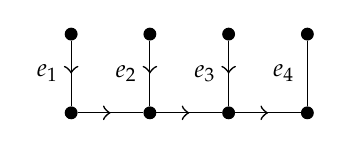
\begin{tikzpicture}[decoration={
        markings,
        mark=at position 0.5 with {\arrow[scale=1.5]{>}}}
      ]
        \foreach \i in {1,...,4}{
          \node[classic] (a\i) at (\i,0) {};
          \node[classic] (b\i) at (\i,1) {};
          \node at (\i-.3,.5) {\small $e_\i$};
        }
        
        \draw[postaction={decorate}] (a1) -- (a2);
        \draw[postaction={decorate}] (a2) -- (a3);
        \draw[postaction={decorate}] (a3) -- (a4);
        
      \draw[postaction={decorate}] (b1) -- (a1);
      \draw[postaction={decorate}] (b2) -- (a2);
      \draw[postaction={decorate}] (b3) -- (a3);
      \draw (b4) -- (a4);
          
      \end{tikzpicture}
      \caption{A valid orientation of $C_i$. The edge $e_1$ is negative, $e_2$ and
        $e_3$ are negative, and $e_4$ can eihter be positive or negative.}
      \label{fig:variable_gadget}
    \end{figure}
  \end{poc}

  \paragraph{Equivalence of the instances}
  We are now ready to prove that $\phi$ admits a valuation such that each
  clause contains true and false variables with different values if and only if
  $G_\phi$ is a $k$-iterated shift graph. More precisely, we prove that if
  $\phi$ admits so such valuation, then $G_\phi$ is not even a shift graph.

  We first prove the reverse implication. Consider a valid orientation of
  $G_\phi$. For each variable $x$, assign $x$ to true if $w^{0}_x \to v^0_x$ and
  to false otherwise. By construction and by \cref{cl:gadget_orientation}, each
  of the edges $e_1, \ldots, e_4$ attached to the internal vertices of $N_i$ is
  positive if and only if the corresponding variable is true. By
  \cref{cl:clause_orientation}, the edges $e_1, \ldots, e_4$ cannot be all
  positive or all negative because the orientation is valid. Hence
  $i$\textsuperscript{th} clause contains a true and a false variable, which
  concludes the proof.


  We now prove the direct implication. Consider such a valuation. With a slight
  abuse of notation, we will name the directed graph arising from the
  progressive orientations of our gadgets with the same naming conventions. For
  each variable $x$, choose the orientation of $M_x$ such that
  $w^{0}_x \to v^{0}_x$ if $x$ is true (by \cref{cl:gadget_orientation} there
  exists only one such orientation). Then orient each copy of the four-sun such
  that each $t^{2i}_x$ has in and outdegree equal to two (by
  \cref{cl:sun_orientation}, there exists a unique such orientation for each
  $(x,i)$). The orientation of each variable gadget $L_x$ is drawn on
  \cref{fig:oriented_variable}.

    \begin{figure}[h!]
    \centering
    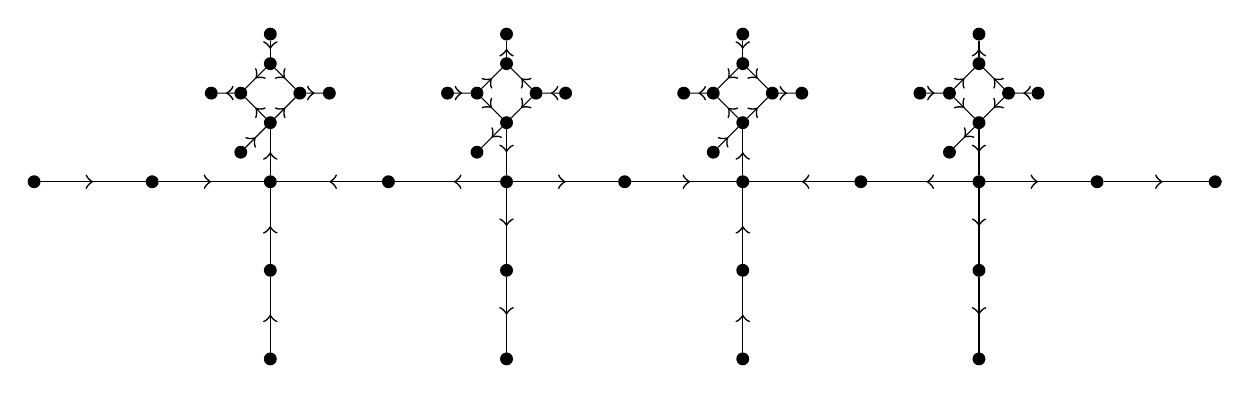
\begin{tikzpicture}[scale = 1.5,decoration={
        markings,
        mark=at position 0.5 with {\arrow[scale=1.5]{>}}}
      ]
      \foreach \i in {0,2}{
        \begin{scope}[shift={(2*\i,0)}]
          \node[classic] (a\i) at (0,0) {};
          
          \node[classic] (e\i1) at (0,-.75) {};
          \node[classic] (e\i2) at (0,-1.5) {};

          \node[classic] (H\i11) at (0,.5) {};
          \node[classic] (H\i12) at (-.25,.25) {};
          \node[classic] (H\i21) at (.25,.75) {};
          \node[classic] (H\i22) at (.5,.75) {};
          \node[classic] (H\i31) at (0,1) {};
          \node[classic] (H\i32) at (0,1.25) {};
          \node[classic] (H\i41) at (-.25,.75) {};
          \node[classic] (H\i42) at (-.5,.75) {};
          \draw[postaction={decorate}] (H\i11) to (H\i21);
          \draw[postaction={decorate}] (H\i11) to (H\i41);
          \draw[postaction={decorate}] (H\i31) to (H\i21);
          \draw[postaction={decorate}] (H\i31) to (H\i41);
          \draw[postaction={decorate}] (e\i1) to (a\i);
          \draw[postaction={decorate}] (a\i) to (H\i11);
          \draw[postaction={decorate}] (e\i2) to (e\i1);
          \foreach \j in {1,3}{
            \draw[postaction={decorate}] (H\i\j2) to (H\i\j1);
          }
          \foreach \j in {2,4}{
            \draw[postaction={decorate}] (H\i\j1) to (H\i\j2);
          }
        \end{scope}                
      }

      \foreach \i in {1,3}{
        \begin{scope}[shift={(2*\i,0)}]
          \node[classic] (a\i) at (0,0) {};
          
          \node[classic] (e\i1) at (0,-.75) {};
          \node[classic] (e\i2) at (0,-1.5) {};

          \node[classic] (H\i11) at (0,.5) {};
          \node[classic] (H\i12) at (-.25,.25) {};
          \node[classic] (H\i21) at (.25,.75) {};
          \node[classic] (H\i22) at (.5,.75) {};
          \node[classic] (H\i31) at (0,1) {};
          \node[classic] (H\i32) at (0,1.25) {};
          \node[classic] (H\i41) at (-.25,.75) {};
          \node[classic] (H\i42) at (-.5,.75) {};
          \draw[postaction={decorate}] (H\i21) to (H\i11);
          \draw[postaction={decorate}] (H\i21) to (H\i31);
          \draw[postaction={decorate}] (H\i41) to (H\i11);
          \draw[postaction={decorate}] (H\i41) to (H\i31);
          \draw[postaction={decorate}] (H\i11) to (a\i);
          \draw[postaction={decorate}] (a\i) to (e\i1);
          \draw[postaction={decorate}] (e\i1) to (e\i2);
          \foreach \j in {2,4}{
            \draw[postaction={decorate}] (H\i\j2) to (H\i\j1);
          }
          \foreach \j in {1,3}{
            \draw[postaction={decorate}] (H\i\j1) to (H\i\j2);
          }
          
        \end{scope}        
        
      }


      \node[classic] (a) at (-2,0) {};
      \node[classic] (b) at (-1,0) {};
      \node[classic] (a4) at (8,0) {};

      \draw[postaction={decorate}] (a) to (b);
      \draw[postaction={decorate}] (b)-- (a0);

      \foreach \i in {1,3}{
        \node[classic] (b\i) at (2*\i+1,0) {};
        \pgfmathsetmacro{\j}{\i+1}
        \draw[postaction={decorate}] (a\i) to (b\i);
        \draw[postaction={decorate}] (b\i)to (a\j);
      }
      \foreach \i in {0,2}{
        \node[classic] (b\i) at (2*\i+1,0) {};
        \pgfmathsetmacro{\j}{\i+1}
        \draw[postaction={decorate}] (a\j) to (b\i);
        \draw[postaction={decorate}] (b\i)to (a\i);
      }
      
       \end{tikzpicture}  
    \caption{The orientation of $L_x$ when $x$ is true (for the false variables,
    the orientation is reversed)}
    \label{fig:oriented_variable}    
  \end{figure}
  
  The only edges that remain to be oriented are the edges forming the spine of
  each clause gadget. Consider the comb $C_i$ corresponding to the
  $i$\textsuperscript{th} clause of $\phi$, with $e_1,\ldots, e_4$ the edges attached to the
  spine of $C_i$. By construction and
  \cref{cl:gadget_orientation}, $e_2$ and $e_3$ are either both negative or both
  positive. Since each clause contains true and false variables, we can apply
  \cref{cl:clause_orientation} to orient the spine of $C_i$. The
  orientation we constructed is valid when restricted to each $C_i$ and to each
  $L_x$. To check that is forms a valid orientation of $G_\phi$, we only need to
  check the first condition of \cref{lem:forbidden_config} at the junctions
  between the clause and the variable gadgets, and the orientation of the cycles
  using these junctions. Note that any such cycle must pass by some $u^{2i}_x$,
  at which it alternates. Finally, as each $u^{2i}_xv^{2i}_xw^{2i}_x$ forms a
  non-alternating path, the first condition of \cref{lem:forbidden_config} is
  satisfied and the orientation of $G_\phi$ is that of an acyclic line
  digraph. In other words, $G_\phi$ is a shift graph. This concludes the proof
  for shift graphs, but not for iterated shift graphs.

  To prove that $G_\phi$ is a $k$-iterated shift graph, we construct an oriented
  acyclic graph $G_\phi'$ such that $G_\phi$ is an induced subgraph of
  $L^k(G_\phi')$. For each variable $x$, by \cref{lem:shift_tree}, there exists
  a graph $M'_x$ with a convex $k$-shift embedding $\psi_x$ of $M_x$ in $M'_x$.
  By \cref{lem:shift_tree}, for each clause comb $C_i$, there exists a
  graph $C'_i$ with a convex $k$-shift embedding $\psi_i$ of $C_i$ in
  $C'_i$. Denote $\psi$ the union of these $k$-shift embedding.

  First, we note that $(\psi(N(v^{2i}_x)))_{i,x}$ forms a collection of pairwise
  disjoint $k+2$-paths because any distinct $v^{2i}_x$ and $v^{2j}_y$ are
  either in different component of the support of $L_x$, or connected by a
  unique path $P$ containing a directed subpath of length $k+2$ between
  $v^{2i}_x$ and $u^{2i}_x$. As result, $\psi(N(v^{2i}_x))$ and $\psi(u^{2i}_x)$
  are vertex disjoint and since $\psi$ is convex, so are the extremities of $P$:
  $\psi(N(v^{2i}_x))$ and $\psi(N(v^{2j}_y))$. By iteratively applying
  \cref{lem:gluing} to identify the leaves of the gadgets $N_i$ to the gadget
  variables along the concerned vertices $v^{4i+2c}_x$ for some $c$, the images
  of the vertices to be indentified remain disjoint. At the end of
  this identification process, we have a $k$-shift embedding of $G_\phi$ minus
  the 4-suns.

  Finally, we identify each $\psi(t^{4i}_x)$ with the path of length $k$
  starting in the vertex $t$ of the graph $F$ drawn on \cref{fig:sun_root}. It
  is straightforward to check that the $k$-line digraph of the graph drawn on
  \cref{fig:sun_root} is the 4-sun and the resulting graph $G'_\phi$ is such
  that $G_\phi$ is an induced subgraph of $G'_\phi$.
  \begin{figure}[h!]
    \centering
    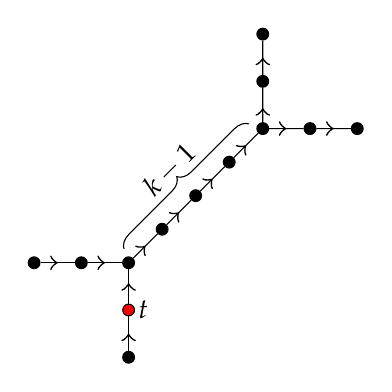
\begin{tikzpicture}[scale = .6,decoration={
        markings,
        mark=at position 0.5 with {\arrow[scale=1.5]{>}}}]
          
      \node[classic] (a1) at (-2,0) {};
      \node[classic] (a2) at (-1,0) {};
      \node[classic] (a3) at (0,0) {};
     
      \node[classic] (b1) at (0,-2) {};
      \node[classic, fill=red] (b2) at (0,-1) {};
      \node[right=0cm] at (b2) {$t$};
  
      \coordinate (b3) at (a3);

      \foreach \i in {1,...,3}{
        \node[classic] (v\i) at (0.71*\i,0.71*\i) {};
      }

      \begin{scope}[shift={(2.84,2.84)}]
        \node[classic] (c1) at (2,0) {};
        \node[classic] (c2) at (1,0) {};
        \node[classic] (c3) at (0,0) {};
        
        \node[classic] (d1) at (0,2) {};
        \node[classic] (d2) at (0,1) {};
        \coordinate (d3) at (c3);
      \end{scope}

      \foreach \u in {a,b}{
        \draw[postaction={decorate}] (\u1) to (\u2);
        \draw[postaction={decorate}] (\u2) to (\u3);
      }
      \foreach \u in {c,d}{
        \draw[postaction={decorate}] (\u3) to (\u2);
        \draw[postaction={decorate}] (\u2) to (\u1);
      }

      \draw[postaction={decorate}] (a3) to (v1);
      \draw[postaction={decorate}] (v1) to (v2);
      \draw[postaction={decorate}] (v2) to (v3);
      \draw[postaction={decorate}] (v3) to (c3);

      \draw [decorate,decoration={brace,amplitude=5pt,mirror,raise=1ex}] (c3) -- (a3) node[midway,xshift=-2ex,yshift=2ex,rotate=45]{$k-1$};
    \end{tikzpicture}  
    \caption{A graph $F$ whose $k$-line digraph is the $4$-sun.}
    \label{fig:sun_root}    
  \end{figure}
\end{proof}


\section*{Acknowledgements}
The research was initiated during a one-week research visit by Nicolas Trotignon
at Jagiellonian University in January 2025, supported by the grant FILL.

\nocite{*}
\bibliographystyle{abbrv}
\bibliography{references}

% \appendix
% \section{Code use for the computer check of \cref{thm:3col}}\label{sec:computer_check}
% To check that all 3-arc-colourings of $H$ colour the two arcs entering $x$ with
% different colours, we compute the number of 3-colourings of $L(H)$ and the
% number of 3-colourings of $G$, where $G$ is obtained from $L(H)$ by
% adding an edge betwenn the vertices correspoding to arcs entering $x$ in
% $H$. The following code shows that these numbers are equal, so all 3-colourings
% of $L(H)$ are 3-colourings of $G$, which implies the desired result.
% \begin{lstlisting}[language=Python]
% from sage.graphs.graph_coloring import chromatic_number, number_of_n_colorings

% # Constructing L(H)
% vertices = [(i,j) for i in range(7) for j in range(i+1,7) if j-i <= 4]
% for i in [3,4]:
%     vertices.append((i,7))
% for i in [5,6]:
%     vertices.append((i,9))  # the vertex x of H is labelled 9 here
% for i in [4,5,6]:
%     vertices.append((i,8))
% d =dict()
% for u in vertices: 
%     L = [v for v in vertices if (v[1] == u[0] or v[0] == u[1])] 
%     d[u] = L
% LH = Graph(d)

% # Computing the number of 3-colourings
% print("L(H) has " + str(number_of_n_colorings(LH,3)) + " proper 3-colourings")
% LH.add_edge((6,9),(5,9)) # LH is now the graph G
% print("G has " + str(number_of_n_colorings(LH,3)) + " proper 3-colourings")
% \end{lstlisting}

\end{document}

